\documentclass{article}
\usepackage[hyphens]{url}
\usepackage{mathtools}
\usepackage{amsmath}
\usepackage{listings}
\usepackage{graphicx}
\usepackage[margin=1in]{geometry}
\usepackage{float}
\floatstyle{boxed}
\restylefloat{figure}
\lstset{basicstyle=\footnotesize, breaklines=true}
\begin{document}


\title{CS595 Intro to Web Science, Assignment \#10}
\author{Valentina Neblitt-Jones}
\date{December 12, 2013}
\maketitle

\newpage
%\listoftables
\lstlistoflistings
\listoffigures

\newpage
\section*{Question 1}

Choose a blog or newsfeed (or something with an Atom or RSS feed). It should be on a topic or topics or which you are qualified to provide classification training data. Find something with at least 100 entries. \\

Create between four and eight different categories for the entries in the feed: \\

examples: \\

work, class, family, news, deals \\

liberal, conservative, moderate, libertarian \\

sports, local, financial, national, international, entertainment \\

metal, electronic, ambient, folk, hip-hop, pop \\

Download and process the pages of the feed as per the week 12 class slides.

\subsection*{Answer to Question 1}

Since I am an adult fan of LEGO (AFOL), I looked for a blog about LEGO and found \textit{Gimme LEGO: The musing of a LEGO obsessive} at \url{http://gimmelego.blogspot.com/} (Figure \ref{gimmelegopage}). I am a founding member of a local LEGO club (HARDLUG) that has existed for 11 years and feel qualified to classify a blog about the hobby/obsession. \\

My categories were the following:

\begin{itemize}
\item original - originals meaning not a set; the correct term is MOC meaning ``my own creation'', but I felt that was unreasonable use of jargon
\item sets - official sets release by The LEGO Group
\item events - launch events, tours or conferences attended by the blogger
\item awards - awards either in the blogger's opinion or his readers' opinions
\item minifigures - focused on LEGO mini figures; The LEGO Group started releasing collectible minifigures in series in 2010
\item market - posts about prices whether it was about deals/bargains or complaints
\item summary - infrequently the blogger would write about blogging about LEGO and how it was going so far (e.g., successes, failures)
\end{itemize}

I believe these categories are suitable for a general audience. If my audience was other AFOLs, I would be more detailed and specific with my subject headings. \\

\begin{figure}[H]
\centering
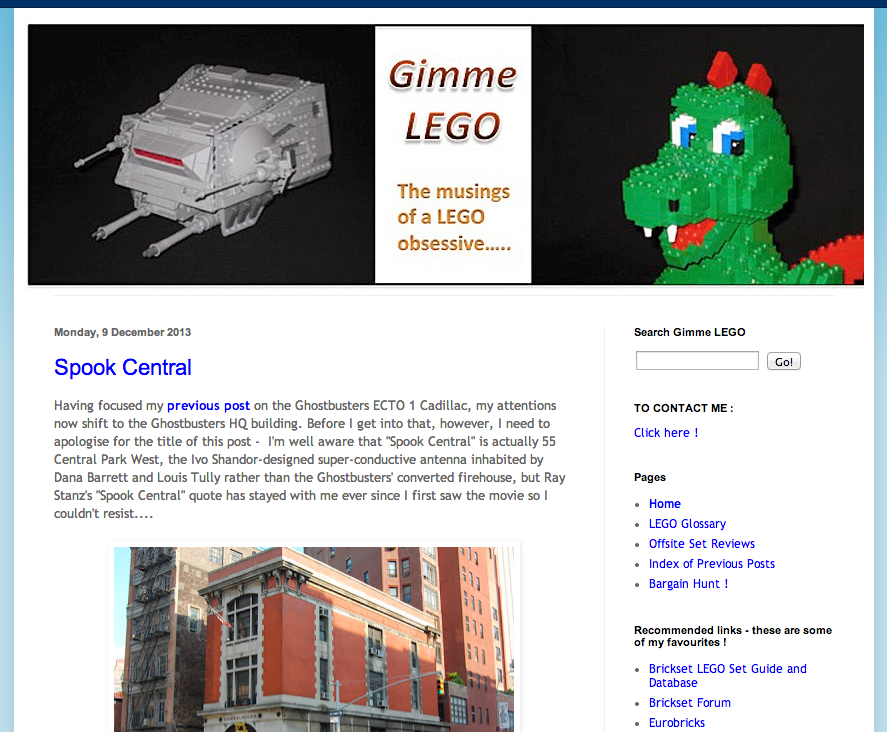
\includegraphics[scale=0.50]{files/gimmelegopage}
\caption{Gimme LEGO Blog}
\label{gimmelegopage}
\end{figure}

To obtain the XML file with the 100 entries, I clicked on the link to subscribe to posts via Atom and changed the max results to 100 (\url{http://gimmelego.blogspot.com/feeds/posts/default?max-results=100}) and saved the file as xml. The file is titled gimmelego.xml on GitHub at \url{https://github.com/vneblitt/cs595-f13/blob/master/assignment10/files/gimmelego.xml}. The blog titles are in Appendix C.



%\begin{figure}[H]
%\centering
%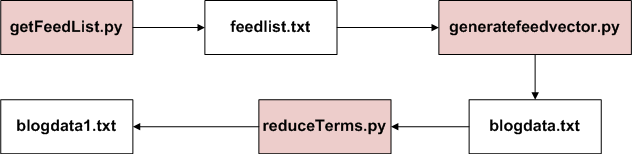
\includegraphics[scale=0.50]{q01/FlowForQ1}
%\caption{Creation of the Blog-Term Matrix}
%\label{FlowForQ1}
%\end{figure}

\newpage
\section*{Question 2}
Manually classify the first 50 entries, and then classify (using the fisher classifier) the remaining 50 entries. Report the cprob() values for the 50 titles as well. From the title or entry itself, specify the 1-, 2-, or 3-gram that you used for the string to classify. Do not repeat strings; you will have 50 unique strings. For example, in these titles the string used is marked with *s: \\

\begin{itemize}
\item *Rachel Goswell* - ``Waves are Universal'' (LP Review)
\item The *Naked and Famous* - ``Passive Me, Aggressive You'' (LP Review)
\item *Negativland* - ``Live at Lewis's, Norfolk VA, November 21, 1992'' (concert)
\item Negativland - ``*U2*'' (LP Review)
\end{itemize}

Note how 	``Negativland'' is not repeated as a classification string. \\

Create a table with the title, the string used for classification, cprob(), predicted category, and actual category.

\subsection*{Answer to Question 2}

This was disappointing. I managed to manually classify the first 50 entries and generate the database file using createTrainingData.py and docclass.py\cite{pci} (Listings \ref{createtrainingdata} and \ref{docclass}). The database is on GitHub and titled gimmelego.db. My next set of error messages indicated that my program could not access the generated database to classify the second 50 entries. I do hope to eventually figure it out.

%\begin{lstlisting}[frame=single, caption=generateImages.py, label=generateImages]
%\end{lstlisting}

%\begin{table}[!h]
%\centering
%\begin{tabular}{c c}
%Value of k & No. of Iterations \\
%\hline
%5 & 6  \\
%10 & 7  \\
%20 & 100  \\
%\hline
%\end{tabular}
%\caption{K-Means Iterations}
%\end{table}

\newpage
\section*{Question 3}

Assess the performance of your classifier in each of your categories by computing precision and recall. Note that the definitions are slightly different in the context of classification; see: \url{http://en.wikipedia.org/wiki/Precision_and_recall#Definition_.28classification_context.29}

\subsection*{Answer to Question 3}

Not reached due to problems with Q2.

%\begin{lstlisting}[frame=single, caption=getKMeans.py, label=getKMeans]
%\end{lstlisting}

%\begin{itemize}
%\item Blonde Ambition
%\item ups
%\item Alcorn Studios
%\item All Scattered
%\end{itemize}

\newpage

\section*{Question 4 - Extra Credit (5 points)}

Redo the questions above, but with the extensions on slide 26 and pp. 136-138.

\subsection*{Answer to Question 4}

Not attempted.

%\renewcommand\thesubsection{\arabic{subsection}}
%\subsection{What 5 movies have the highest average ratings? Show the movies and their ratings sorted by their average ratings.}

%\begin{lstlisting}[frame=single, caption=highestavgrating.py, label=highaverage]
%\end{lstlisting}

%\newpage
%\subsection{What 5 movies have received the most ratings? Show the movies and the number of ratings sorted by number of ratings.}

%\begin{table}[!h]
%\centering
%\begin{tabular}{l c}
%Movie Title & No. of Ratings \\
%\hline
%Star Wars (1977) & 583  \\
%Contact (1997) & 509  \\
%Fargo (1996) & 508  \\
%Return of the Jedi (1983) & 507  \\
%Marlene Dietrich: Shadow and Light (1997) & 485  \\
%\hline
%\end{tabular}
%\caption{Movies with the Most Ratings}
%\end{table}

%\begin{figure}[H]
%\centering
%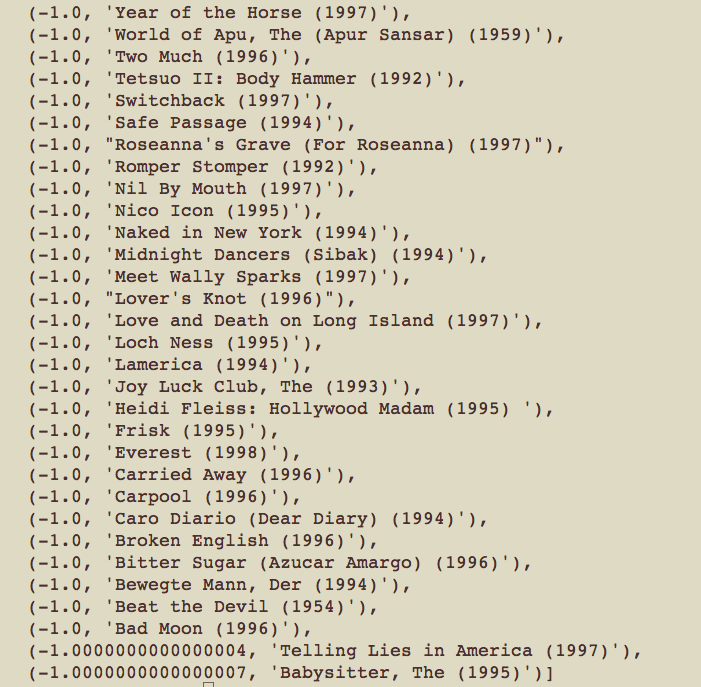
\includegraphics[scale=0.50]{q05/leastliketopgun}
%\caption{Movies Least Like Top Gun}
%\label{leastliketopgun}
%\end{figure}

\newpage
\appendix

\section{createTrainingData.py}

\begin{lstlisting}[frame=single, caption=createTrainingData.py, label=createtrainingdata]
import os
import feedparser
import docclass

os.unlink(`gimmelego.db')

# The first 50 entries manually classified
cl=docclass.classifier(docclass.getwords)

cl.setdb(`gimmelego.db')

d = feedparser.parse(`http://gimmelego.blogspot.com/feeds/posts/default?max-results=100')

cl.train(d.entries[0].content[0].value, `original')
cl.train(d.entries[1].content[0].value, `original')
cl.train(d.entries[2].content[0].value, `books')
cl.train(d.entries[3].content[0].value, `sets')
cl.train(d.entries[4].content[0].value, `events')
cl.train(d.entries[5].content[0].value, `events')
cl.train(d.entries[6].content[0].value, `original')
cl.train(d.entries[7].content[0].value, `sets')
cl.train(d.entries[8].content[0].value, `sets')
cl.train(d.entries[9].content[0].value, `books')
cl.train(d.entries[10].content[0].value, `events')
cl.train(d.entries[11].content[0].value, `sets')
cl.train(d.entries[12].content[0].value, `original')
cl.train(d.entries[13].content[0].value, `original')
cl.train(d.entries[14].content[0].value, `events')
cl.train(d.entries[15].content[0].value, `events')
cl.train(d.entries[16].content[0].value, `sets')
cl.train(d.entries[17].content[0].value, `sets')
cl.train(d.entries[18].content[0].value, `minifigures')
cl.train(d.entries[19].content[0].value, `original')
cl.train(d.entries[20].content[0].value, `sets')
cl.train(d.entries[21].content[0].value, `sets')
cl.train(d.entries[22].content[0].value, `sets')
cl.train(d.entries[23].content[0].value, `sets')
cl.train(d.entries[24].content[0].value, `sets')
cl.train(d.entries[25].content[0].value, `original')
cl.train(d.entries[26].content[0].value, `sets')
cl.train(d.entries[27].content[0].value, `original')
cl.train(d.entries[28].content[0].value, `sets')
cl.train(d.entries[29].content[0].value, `awards')
cl.train(d.entries[30].content[0].value, `sets')
cl.train(d.entries[31].content[0].value, `awards')
cl.train(d.entries[32].content[0].value, `awards')
cl.train(d.entries[33].content[0].value, `sets')
cl.train(d.entries[34].content[0].value, `sets')
cl.train(d.entries[35].content[0].value, `original')
cl.train(d.entries[36].content[0].value, `sets')
cl.train(d.entries[37].content[0].value, `sets')
cl.train(d.entries[38].content[0].value, `market')
cl.train(d.entries[39].content[0].value, `original')
cl.train(d.entries[40].content[0].value, `events')
cl.train(d.entries[41].content[0].value, `sets')
cl.train(d.entries[42].content[0].value, `original')
cl.train(d.entries[43].content[0].value, `sets')
cl.train(d.entries[44].content[0].value, `minifigures')
cl.train(d.entries[45].content[0].value, `original')
cl.train(d.entries[46].content[0].value, `summary')
cl.train(d.entries[47].content[0].value, `original')
cl.train(d.entries[48].content[0].value, `sets')
cl.train(d.entries[49].content[0].value, `market')

# The second 50 entries classified using Fisher

cl = docclass.fisherclassifier(docclass.getwords)

for i in range(50, 100):
	category = cl.classify(d.entries[i].content[0].value)
	print d.entries[i].title + ` : ' + category
	
for i in range(50, 100):
	for cat in categories:
		print cl.cprob(d.entries[i].title, cat)

\end{lstlisting}

\section{docclass.py}

\begin{lstlisting}[frame=single, caption=docclass.py, label=docclass]
from pysqlite2 import dbapi2 as sqlite
import re
import math

def getwords(doc):
  splitter=re.compile(`\`\\W*')
  print doc
  # Split the words by non-alpha characters
  words=[s.lower() for s in splitter.split(doc) 
          if len(s)>2 and len(s)<20]
  
  # Return the unique set of words only
  return dict([(w,1) for w in words])

class classifier:
  def __init__(self,getfeatures,filename=None):
    # Counts of feature/category combinations
    self.fc={}
    # Counts of documents in each category
    self.cc={}
    self.getfeatures=getfeatures
    
  def setdb(self,dbfile):
    self.con=sqlite.connect(dbfile)    
    self.con.execute(`create table if not exists fc(feature,category,count)')
    self.con.execute(`create table if not exists cc(category,count)')


  def incf(self,f,cat):
    count=self.fcount(f,cat)
    if count==0:
      self.con.execute(``insert into fc values (`%s',`%s',1)" 
                       % (f,cat))
    else:
      self.con.execute(
        ``update fc set count=%d where feature=`%s' and category=`%s'" 
        % (count+1,f,cat)) 
  
  def fcount(self,f,cat):
    res=self.con.execute(
      `select count from fc where feature=``%s" and category=``%s"'
      %(f,cat)).fetchone()
    if res==None: return 0
    else: return float(res[0])

  def incc(self,cat):
    count=self.catcount(cat)
    if count==0:
      self.con.execute(``insert into cc values (`%s',1)" % (cat))
    else:
      self.con.execute(``update cc set count=%d where category=`%s'" 
                       % (count+1,cat))    

  def catcount(self,cat):
    res=self.con.execute(`select count from cc where category=``%s"'
                         %(cat)).fetchone()
    if res==None: return 0
    else: return float(res[0])

  def categories(self):
    cur=self.con.execute(`select category from cc');
    return [d[0] for d in cur]

  def totalcount(self):
    res=self.con.execute(`select sum(count) from cc').fetchone();
    if res==None: return 0
    return res[0]


  def train(self,item,cat):
    features=self.getfeatures(item)
    # Increment the count for every feature with this category
    for f in features:
      self.incf(f,cat)

    # Increment the count for this category
    self.incc(cat)
    self.con.commit()

  def fprob(self,f,cat):
    if self.catcount(cat)==0: return 0

    # The total number of times this feature appeared in this 
    # category divided by the total number of items in this category
    return self.fcount(f,cat)/self.catcount(cat)

  def weightedprob(self,f,cat,prf,weight=1.0,ap=0.5):
    # Calculate current probability
    basicprob=prf(f,cat)

    # Count the number of times this feature has appeared in
    # all categories
    totals=sum([self.fcount(f,c) for c in self.categories()])

    # Calculate the weighted average
    bp=((weight*ap)+(totals*basicprob))/(weight+totals)
    return bp




class naivebayes(classifier):
  
  def __init__(self,getfeatures):
    classifier.__init__(self,getfeatures)
    self.thresholds={}
  
  def docprob(self,item,cat):
    features=self.getfeatures(item)   

    # Multiply the probabilities of all the features together
    p=1
    for f in features: p*=self.weightedprob(f,cat,self.fprob)
    return p

  def prob(self,item,cat):
    catprob=self.catcount(cat)/self.totalcount()
    docprob=self.docprob(item,cat)
    return docprob*catprob
  
  def setthreshold(self,cat,t):
    self.thresholds[cat]=t
    
  def getthreshold(self,cat):
    if cat not in self.thresholds: return 1.0
    return self.thresholds[cat]
  
  def classify(self,item,default=None):
    probs={}
    # Find the category with the highest probability
    max=0.0
    for cat in self.categories():
      probs[cat]=self.prob(item,cat)
      if probs[cat]>max: 
        max=probs[cat]
        best=cat

    # Make sure the probability exceeds threshold*next best
    for cat in probs:
      if cat==best: continue
      if probs[cat]*self.getthreshold(best)>probs[best]: return default
    return best

class fisherclassifier(classifier):
  def cprob(self,f,cat):
    # The frequency of this feature in this category    
    clf=self.fprob(f,cat)
    if clf==0: return 0

    # The frequency of this feature in all the categories
    freqsum=sum([self.fprob(f,c) for c in self.categories()])

    # The probability is the frequency in this category divided by
    # the overall frequency
    p=clf/(freqsum)
    
    return p
  def fisherprob(self,item,cat):
    # Multiply all the probabilities together
    p=1
    features=self.getfeatures(item)
    for f in features:
      p*=(self.weightedprob(f,cat,self.cprob))

    # Take the natural log and multiply by -2
    fscore=-2*math.log(p)

    # Use the inverse chi2 function to get a probability
    return self.invchi2(fscore,len(features)*2)
  def invchi2(self,chi, df):
    m = chi / 2.0
    sum = term = math.exp(-m)
    for i in range(1, df//2):
        term *= m / i
        sum += term
    return min(sum, 1.0)
  def __init__(self,getfeatures):
    classifier.__init__(self,getfeatures)
    self.minimums={}

  def setminimum(self,cat,min):
    self.minimums[cat]=min
  
  def getminimum(self,cat):
    if cat not in self.minimums: return 0
    return self.minimums[cat]
  def classify(self,item,default=None):
    # Loop through looking for the best result
    best=default
    max=0.0
    for c in self.categories():
      p=self.fisherprob(item,c)
      # Make sure it exceeds its minimum
      if p>self.getminimum(c) and p>max:
        best=c
        max=p
    return best
\end{lstlisting}

\section{100 Blog Titles from GimmeLEGO}

\begin{enumerate}
\item Spook Central
\item Who Ya Gonna Call ?
\item American Beauty
\item A Wretched Hive of Scum and Villainy....
\item STEAMrollered
\item Full STEAM Ahead
\item Gerry Anderson Returns....?
\item Shanghai Surprise
\item Galaxy Squad - Like a Prayer
\item Spoiled for Choice
\item Ready for Launch
\item Designer Robot
\item UCS AT-AT : They think it's all over...
\item UCS AT-AT : The Home Straight
\item LEGO Inside Tour 2013 part 2
\item LEGO Inside Tour 2013
\item Rocky Horror ?
\item Yellows !
\item Gold Rush
\item UCS AT-AT : Raising the Roof
\item Jabba Dabba Doo !
\item Hi Ho Silver Lining
\item Cowabunga !
\item Night at the Museum
\item A-wing and a Prayer
\item UCS AT-AT : Beside Myself...
\item The Real Classic Space ?
\item UCS AT-AT : Heady Days
\item Technic Temptation....
\item ``And the Gimme LEGO Readers' Choice Award for Best Set of 2012 goes to...."
\item Moonlighting
\item 2012 Readers Choice Award - the Nominations
\item The Gimme LEGO Awards 2012
\item ``They're for sale if you want them"
\item One Hundred Percent
\item UCS AT-AT : Once More Unto the Breach....
\item Monsters, Inc.
\item Blast from the Past : Set 657 Executive Jet
\item Bargain Hunt Lives !
\item UCS AT-AT : Body Beautiful
\item Blown Away
\item Van-tastic
\item UCS AT-AT : Tricky
\item Bling
\item Still Going Strong
\item UCS AT-AT : the build begins....
\item Happy Birthday to Me !
\item Building the Perfect Beast - Anatomy of an AT-AT
\item Going for Gold
\item Scalpers Rejoice !
\item Building the Perfect Beast - the UCS AT-AT
\item Hell's Bells
\item Ancient Treasures
\item I Want My Mummy !
\item New York, New York
\item What's that coming over the hill....?
\item Block-tastic
\item Dangerous
\item Spaced Out
\item Fangs for the Memories...
\item Home Truths
\item No Consolation
\item United in Manchester
\item Blast from the Past : Set 695 Racing Car
\item Dreams Can Come True...
\item Apologies...
\item Headache
\item Whoops...
\item 3-in-1
\item Sneak Peek part 2 : Star Wars Miniland
\item Sneak Peek
\item ``The damage doesn't look as bad from out here"
\item Baubles
\item So Bad it's Almost Good
\item Once upon a time......
\item The Joy of Six
\item Dino
\item A Different World
\item One step back and two steps forward....
\item Taking the Plunge
\item The 2011 Gimme LEGO Readers Choice Award.....
\item Christmas Car-nage
\item 25th of December it is.....
\item The Gimme LEGO Awards 2011
\item The best things....
\item Better late than never
\item Shuttle Love
\item Bucket List Reloaded
\item Bucket List
\item Charidee
\item Girl's Stuff
\item Blasphemy
\item Here comes The Sun
\item Here there be Dragons...
\item One Year On....
\item Revealed : Kingdoms Set 10223 Royal Joust
\item Midi-chlorians
\item Neo- Neo- Classic Space ?
\item Favourite Sets \#6 : Tractor
\item Ultimate ?
\end{enumerate}

\newpage

\bibliographystyle{acm}
\bibliography{references}

\end{document}